\documentclass[a4paper,12pt]{article}
%DIF LATEXDIFF DIFFERENCE FILE
%DIF DEL msc_szakdolgozat_master.tex   Tue May  3 14:43:41 2016
%DIF ADD msc_szakdolgozat.tex          Tue May  3 16:16:51 2016

%temporary includes
\usepackage{textcomp} %for arrows in comments

% Remove colours from refs%
\usepackage[hidelinks]{hyperref}

%includes
\usepackage{color}
\usepackage{cite}

% magyar nyelv
\usepackage[magyar]{babel}
\usepackage[utf8]{inputenc}

\usepackage{fixltx2e}
\usepackage{hyperref}

% for pseudocode
 \usepackage{algorithm2e}

% for set notation
\usepackage{mathbbol}

% for matrices
\usepackage{amsmath}
\usepackage{blkarray}

% for images
\usepackage{graphicx}
\usepackage{float}
\graphicspath{ {img/} }
\usepackage{sidecap}

\DeclareUnicodeCharacter{00A0}{ }
%\DeclareUnicodeCharacter{00A0}{~} % not using no-break space

% sizes
\usepackage{geometry}
\geometry{
    left=25mm,
    right=25mm,
    top=25mm,
    bottom=25mm,
}
% sorköz
\linespread{1.5}

% For tables
\usepackage{array}
\usepackage{calc}

% Equation description
\usepackage{enumitem}

% Adding dots after section numbers
\usepackage{titlesec}
\titlelabel{\thetitle.\quad}


\pdfinfo{%
  /Title    (Bakteriális patogén és ember közötti molekuláris hálózatok vizsgálata)
  /Author   (Horváth Balázs)
  /Creator  ()
  /Producer ()
  /Subject  (MSc Szakdolgozat)
  /Keywords ()
}

%Title page
%TODO: add more information, logo and stuff as requested
\title{Bakteriális patogén és ember közötti molekuláris hálózatok vizsgálata}
\author{Horváth Balázs}
\date{2015}
%DIF PREAMBLE EXTENSION ADDED BY LATEXDIFF
%DIF UNDERLINE PREAMBLE %DIF PREAMBLE
\RequirePackage[normalem]{ulem} %DIF PREAMBLE
\RequirePackage{color}\definecolor{RED}{rgb}{1,0,0}\definecolor{BLUE}{rgb}{0,0,1} %DIF PREAMBLE
\providecommand{\DIFaddtex}[1]{{\protect\color{blue}\uwave{#1}}} %DIF PREAMBLE
\providecommand{\DIFdeltex}[1]{{\protect\color{red}\sout{#1}}}                      %DIF PREAMBLE
%DIF SAFE PREAMBLE %DIF PREAMBLE
\providecommand{\DIFaddbegin}{} %DIF PREAMBLE
\providecommand{\DIFaddend}{} %DIF PREAMBLE
\providecommand{\DIFdelbegin}{} %DIF PREAMBLE
\providecommand{\DIFdelend}{} %DIF PREAMBLE
%DIF FLOATSAFE PREAMBLE %DIF PREAMBLE
\providecommand{\DIFaddFL}[1]{\DIFadd{#1}} %DIF PREAMBLE
\providecommand{\DIFdelFL}[1]{\DIFdel{#1}} %DIF PREAMBLE
\providecommand{\DIFaddbeginFL}{} %DIF PREAMBLE
\providecommand{\DIFaddendFL}{} %DIF PREAMBLE
\providecommand{\DIFdelbeginFL}{} %DIF PREAMBLE
\providecommand{\DIFdelendFL}{} %DIF PREAMBLE
%DIF END PREAMBLE EXTENSION ADDED BY LATEXDIFF
%DIF PREAMBLE EXTENSION ADDED BY LATEXDIFF
%DIF HYPERREF PREAMBLE %DIF PREAMBLE
\providecommand{\DIFadd}[1]{\texorpdfstring{\DIFaddtex{#1}}{#1}} %DIF PREAMBLE
\providecommand{\DIFdel}[1]{\texorpdfstring{\DIFdeltex{#1}}{}} %DIF PREAMBLE
%DIF END PREAMBLE EXTENSION ADDED BY LATEXDIFF

\begin{document}
\maketitle
\pagebreak

\section{Tartalomjegyzék}
\pagebreak

\section{Rövidítésjegyzék}
PPI - protein protein interaction
\pagebreak

\section{Bevezetés}
	\subsection{A bél mikrobióta fontosságának ismertetése}
		\paragraph{Miért van szükség a bél mikrobióta vizsgálatára?} \mbox{}\\
		A humán bél mikrobióta egy komplex ökoszisztéma. A mikrobiomot alkotó sejtek száma nagyjából a humán szomatikus és csírasejtek összegének tízszerese.  A bél mikrobiom mind metabolikusan, mind immunológiailag komplex kapcsolatban áll az emberrel.\cite{gut_microbiome} Eddig több mint három millió nem redundáns mikrobiális gént sikerült kimutatni az emberben \cite{meta_omics}. Ez a nagy genetikai állomány lehetővé teszi, hogy olyan metabolikus folyamatok játszódjanak le a humán bélben, melyeket az emberi sejtek nem képesek végrehajtani. \cite{gut_microbiome} A bél mikrobióta felelős bizonyos glikánok, aminosavak és xenobiotikumok metabolizmusáért valamint rövid láncú zsírsavak (\textit{short chained fatty acids - SCFA}-k), vitaminok és kofaktorok termeléséért. A gazda által meg nem emésztett poliszacharidok bontását a bél mikrobióta végzi, mely folyamat eredményeképpen olyan rövid láncú zsírsavak keletkeznek mint az acetát, proprionát és vajsav. \cite{scfa_and_vitamine} \\
		\indent		 A bélflóra kulcsszerepet játszik az immun-homeosztázis fenntartásában. Az immunrendszerrel bakteriális mintázatokat észlelő receptorokon keresztül és GPCR-ek által van kapcsolatban. A mikroorganizmusok által termelt SCFA-k képesek GPCR-eken keresztül sejtszignalizáció indítására. A veleszületett immunrendszer nagy részét alkotó monociták és neutrofil granulociták rendelkeznek GPR43 receptorral, mely szintén SCFA érzékeny, tehát a bélflóra metabolitokon keresztül is kapcsolatban áll az immunrendszerrel. \cite{buthyrate_immune} \\
		\indent  A bélflóra hatással van még a gazda metabolizmusára is.  Az \textit{Eubacterium spp.} által oligoszacharidokból képzett vajsav részt vesz az emberi szervezet energia egyensúlyának szabályzásában. \cite{gut_microbiome} Az enteroendokrin sejtek és az adipociták is rendelkeznek a GPR41 receptorral mely vajsavra és proprionátra is érzékeny. Adipocitáknál ez a GPR41 szignalizáció \textit{leptin} elválasztást eredményez. \cite{buthyrate_immune} A vajsav segít a karcinogenezis kivédésében mivel apoptózis indukáló és proliferáció gátló hatása van. Éppen ezen okokból a bél mikrobióta tekinthető egy új metabolikus szervnek is. \cite{host_bacterial_mutualism} Kapcsolatok mutathatók ki a bél mikrobiom megváltozása és olyan betegségek között mint az IBD (\textit{inflammatory bowl disease}), elhízás vagy \DIFdelbegin \DIFdel{a }\DIFdelend \DIFaddbegin \DIFadd{lülönböző }\DIFaddend rák \DIFaddbegin \DIFadd{típusok}\DIFaddend . \cite{gut_microbiome}

		\paragraph{A bél mikrobióta vizsgálatának módszerei} \mbox{}\\
		A mikrobióta vizsgálatát elsősorban a különböző meta omikák eszköztárával közelítik meg. Ezek közül is a \DIFdelbegin \DIFdel{legfőbb }\DIFdelend \DIFaddbegin \DIFadd{legfontosabb }\DIFaddend eszköztár a metagenomika, de alkalmaznak már metabolomikai, metatranszkriptomikai és metaproteomikai megközelítést is. A metagenomikai vizsgálatok során a környezetből származó mintát megfelelő előkészítés után közvetlenül \textit{shotgun} szekvenálásnak vetik alá.\cite{gut_microbiome}

		Quin és \DIFdelbegin \DIFdel{társai2010-re }\DIFdelend \DIFaddbegin \DIFadd{társai 2010-re }\DIFaddend meghatározták a minimális bél metagenomot. A vizsgálat során Illumina GA short-read alapú technológiával 124 egy kohortba tartozó nordikus és mediterrán személy székletmintáját elemezték. Az ebből kinyert 576,7 gigabázásnyi DNS-ből 3,3 millió nem redundáns mikrobiális gént mutattak ki. Az így kimutatott gének az emberi genom százötvenszeresét teszik ki. A minták egészére jellemző, hogy a bennük található gének két fő részre osztható: A legnagyobb csoportba (86\%) a sűrűn előforduló mikrobiális gének, míg a másik fő csoportba pedig a kifejezetten a humán bélflórára jellemző mikrobiális gének tartoznak. Az összes személyből származó vizsgált génhalmaz 99,1\%-a \textit{Eubacteria}, 0,8\%-a \textit{Archea} és a fennmaradó 0,1\%-a pedig vegyesen \textit{Eucaryota} és virális eredetű. A bakteriális eredetű gének összesen 1000-1150 uralkodó baktériumfajhoz tartozhatnak, ami személyenként kb. 160 domináns fajt jelent. A személyekre jellemző nagyjából 160 uralkodó baktériumfaj listái között a személyeket összevetve nagyfokú hasonlóság figyelhető meg. Egy adott személy bél metagenomjának minimálisan 40\%-a megtalálható a minták legalább felében. A közelítőleg ezer fajból 75 faj található meg a minták több mint felében és 57 faj van ami a minták nagyobb mint 90\%-ban kimutatható.  \cite{meta_omics}

	\subsection{A szakirodalomban publikált gazda patogén hálózatok}
	\textcolor{red}{ !TODO}

	\subsection{A Humán-Salmonella kapcsolat ismertetése és hatása az autofágiára}

		\paragraph{\textit{Salmonella spp.}} \mbox{}\\
		A \textit{Salmonell}ák olyan Gram-negatív patogének melyek az állatok széles skáláját képesek fertőzni. A tudomány jelenleg több ezer szerotípust ismer, melyek két fő típusra oszthatók. Az egyik fő típus a \textit{Typhoid}, ebbe a csoportba tartozik a \textit{Typhi} és \textit{Paratyphi} melyek kifejezetten embert fertőznek. A másik fő csoport a \textit{Non-typhoid} amelybe tartozó baktériumok már széleskörű gazdaspecificitással rendelkeznek.

		A fertőzés kontaminált étel vagy folyadék fogyaztásával történik. A \textit{Salmonell}ák az alacsony pH és oxidatív stressz ellen adaptív toleranciával rendelkeznek, így képesek eltűrni a gyomor savasságát és a veleszületett immunrendszer egyéb hatásait. A vékonybélbe jutva az epithélium sejtjeit fertőzik. Fő célpontjaik a \textit{microfold} (\textit{M cells}) sejtek, melyek fő feladata, hogy pinocitózissal mintákat vegyenek a középbél atnigénjeiből és ezt antigén prezentáló sejteknek adják. Azonban a \textit{Salmonell}ák úgynevezett baktérium-közvetített endocítózissal képesek még a nem fagocita típusú enterocitákba is bejutni \cite{salmonella_and_host_cell_nature}


		\paragraph{A \textit{Salmonella} életciklusa} \mbox{}\\
		Az intracelluláris baktériumok életciklusa általánosan három stádiumra osztható: A bejutáshoz használt vakólum elhagyása, replikáció a citoszólban és a citoszólikus veleszületett immunitás elemeinek manipulációja. A \textit{Salmonella} az úgynevezett \textit{trigger} mechanizmussal jut be a sejtbe. A mechanizmus során a baktérium olyan fehérjéket juttat be az eukarióta sejtbe, melyek képesek a sejtvázzal kölcsönhatni. Ezek a bakteriális effektorfehérjék nagyfokú sejtváz-átrendeződést váltanak ki az eukarióta gazdában. A folyamat végén a baktérium egy vakólummal határolva a sejt belsejébe kerül. \cite{salmonella_autophagy_nature_old} Ezt a képletet a szakirodalomban SCV-nek nevezik (\textit{Salmonella containing vacuole}). \cite{salmonella_and_host_cell_nature}

		A fagocitózis végeztével a \textit{Salmonell}ák átesnek egy úgynevezett bakteriális felszín átformázáson (\textit{bacterial surface remodeling}). A folyamat során represszálódnak az olyan bakteriális gének expressziója amit a gazda könnyen fertőzési jelnek tekinthet. Ilyen gének például a SPI1, a T3SS és a flagellin. Mindezek mellett megváltozik a baktériumok felszíni lipopoliszacharid mintázata is.  \cite{salmonella_and_host_cell_nature}

		 \begin{figure}[H]
			 \centering
			 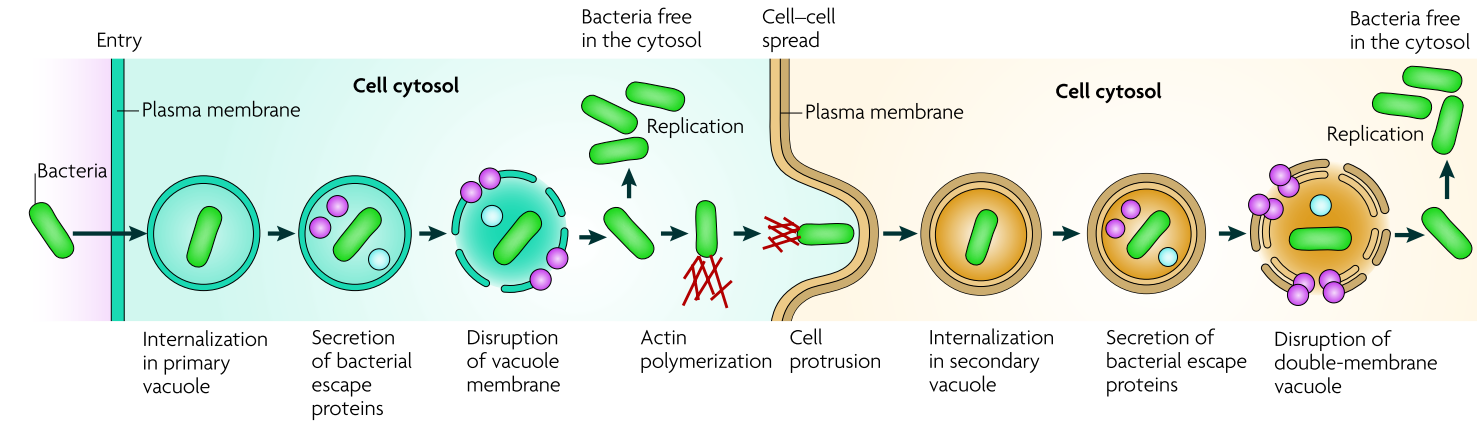
\includegraphics[scale=0.42]{img/salmonella_life_cycle.png}
			 \caption{\textbf{Az intracelluláris baktériumok életciklusa}}
			 Bejutáskor a baktériumok egy elsődleges vakólumba érkeznek. A sejt a belsejében a mikróbák olyan fehérjéket szekretálnak, melyek felbontják az őket határoló elsődleges vakólum membránját. A legtöbb intracelluláris baktériumra jellemző, hogy befolyásolni tudja az aktin polimerizációt és ezáltal képes az intra- és intercelluláris mozgásra. A szomszédos sejtbe átjutott baktériumok egy másdlagos memránburokba kerülnek, melyet ugyancsak felbontanak.
			\textcolor{red}{!TODO kép magyarítás és formázás, jobban látható feliratok}
			 \label{fig:salmo_cycle}
		 \end{figure}

		 Normális körülmények között a vakólum pH-ja mindaddig fokozatosan csökken amíg érett degradatív fagolizoszómává nem válik. A baktériumok kétféleképpen képesek életben maradni ebben a környezetben: A vakólum-lizoszóma fúzió gátlásával, vagy a fagolizoszóma összetételének aktív módosításával. \cite{salmonella_autophagy_nature_old} A szakirodalomban még nincs kialakult álláspont arról, hogy a \textit{Salmonell}ák melyik mechanizmust használják. Bizonyítottan képesek életben maradni, olyan SCV-ben mely már fuzionált a lizoszómával, viszont a fő útvonal valószínűleg a vakólum savanyítási folyamatának késleltetése lehet. \cite{salmonella_and_host_cell_nature}

		 Az SCV-n belül a \textit{S. typhimurium} képes a replikációra. A hármas típusú szekréciós rendszer segítségével a baktériumsejtek olyan anyagokat tudnak kibocsájtani, melyek lehetővé teszik az SCV-ből kijutást és citoplazma invázióját. \cite{salmonella_authopagy_intro}

		 \paragraph{A hármas típusú szekréciós rendszer (T3SS vagy TTSS)} \mbox{}\\
		 A T3SS evolúciósan a flagelláris export rendszerrel mutat rokonságot. Jelenléte esszenciális ahhoz, hogy a \textit{Salmonella} képes legyen a fertőzésre és gazda sejtjeinek kolonizálására. A T3SS felelős a baktérium virulencia vagy effektor fehérjéinek átviteléért. Az effektorok az eukarióta sejtbe jutva megváltoztatják annak sejtfunkcióit. Az virulenciafehérjék átalakítják a gazda citoszkeleton architektúráját, membrán anyagáramlását, szignál transzdukcióját és citokin expresszióját, ezzel segítve a baktériumok túlélését és további kolonizációját. \cite{salmonella_and_host_cell_nature}

		 \paragraph{A \textit{Salmonella} és az autofágia kapcsolata} \mbox{}\\
		 Az autofágia egy intracelluláris katabolikus folyamat melynek szerepe van a fehérjeaggregátumok és károsodott sejtorganellumok eltávolításában és a veleszületett immunrendszer működésében. A \textit{xenofágia} az autofágiának azon formája mely során az intracelluláris baktériumok és vírusok szelektív felismerése és lebontása történik. A szelektív felismerésért az autofágia adaptor fehérjéi felelősek. Ilyen receptor fehérje például a p62 (SQSTM1), a NDP52, optineurin (OPTN) és az NBR1. Az előbb felsorolt receptorok a szubsztrátjuk megkötése után kargo adaptorként viselkednek az LC3 (ATG8) számára. \textit{Salmonella fertőzéskor} a sérült SCV-ből kilépett baktériumok sejtfelszíni fehérjéi poliubiquitin borítást kapnak amit a kargo adaptor fehérjék érzékelnek. \textit{S. typhimurium} fertőzéskor a poliubiquitinált baktériumokat NDP52 és a p62 is felismeri. Az így megkötött baktériumok xenofágia útján eltávolítódnak. \cite{salmonella_authopagy_intro}

	\subsection{Ökológiai hálózatok elemzésére használt topológiai mérőszámok}

	 \paragraph{Miért van szükség topológiai mérőszámokra?} \mbox{}\\ %linebreak after paragraph title
	 A konzervrációs biológia az élettudományok azon ága mely a Föld biodiverzitásának megőrzésével foglalkozik. Mivel az összes faj védelme nem megoldható, ezért szükségessé vált olyan fajok kiválogatása melyek kiemelt figyelmet igényelnek konzervációs biológiai szempontból.\cite{new_zeland} Az 1990-es évek előtt a védelemre való kiválasztás fő szempontja a faj ritkasága volt.  A fajok ilyen alapú szelekciója nem veszi figyelembe hogy például az adott taxon kulcsszerepet játszik-e az ökoszisztéma funkciók ellátásában. \cite{jordan_comparison}

	 \paragraph{Kulcsfajok} \mbox{}\\ %linebreak after paragraph title
	 1966-ban Robert Paine megalkotta a kulcsfaj koncepciót(\textit{keystone species}). Megfigyelte hogy ha kiesik a Kaliforniai sziklás tengerparti közösségből a \textit{Piaster ochraceus} csúcsragadozó tengeri csillag akkor az egész közösség fajösszetétele összeomlik. A mai legelfogadottabb kulcsfaj definíció szerint ezek olyan fajok, melyek ökológiai hatása aránytalanul nagy az abundanciájukhoz képest. A fogalommal kapcsolatban azonban további kérdések merülnek fel: Milyen hatás számít nagynak? Pontosan mekkora biomassza hányad után mondható az adott faj ereje aránytalannak? \cite{new_zeland} Ez utóbbi kérdések megválaszolásához szükség van olyan mérőszámokra, melyek segítségével kvantitatívvé tehető egy adott faj ökológiai fontossága. Másrészt így lehetővé válik a fajkiválasztás során a szubjektivitás csökkentése is. Az ilyen mérőszámok használatával objektív fontossági sorrendet lehet felállítani az adott élőhelyen előforduló taxonok között. \cite{jordan_comparison}

	 \paragraph{Rangsorolásra használt topológiai mérőszámok az ökológiában} \mbox{}\\
	 Ma már a kulcsfajok kiválasztása részben ökológiai interakciós hálózatok elemzése alapján történik. A használt hálók kizárólag biotikus-biotikus (faj-faj) kapcsolatokat tartalmaznak. Erre azért van szükség, mert például minden élőlény összekötésben áll a detritusszal és ez eltorzítaná az analízis eredményét. Sőt ilyen esetben a detritusz maga is struktúrális kulcsfajnak számítana. Egy adott fajnak az ökológiai interakciós hálóban betöltött szerepét pozicionális fontossági mérőszámokkal, vagy más néven centralitási indexekkel lehet jellemezni. A konzervációs biológiában sokfajta ilyen mérőszámot használnak, melyeknek közös tulajdonsága, hogy mindegyik valamilyen egyedi tulajdonságra fekteti a hangsúlyt és az alapján rangsorolja a hálózatban szereplő fajokat. Ilyen eltérés lehet két index között például, az hogy az egyik egy adott pont lokális kapcsolati mintázatára, míg a másik az egész hálózatra vonatkozó hatását számszerűsíti. Adott hálóra különböző mérőszámok eltérő fajsorrendeket adnak, de a hasonló tulajdonságok figyelembevételén alapuló mérőszámok között felállíthatók konszenzus fák. \cite{jordan_comparison}

	 \paragraph{Főbb topológiai mérőszámok}

	 \paragraph{Normalised degree - D} \mbox{}\\Az adott ponttal kapcsolódó pontok száma elosztva a hálózat összes pontjának számával. \cite{top_indexes}

	 \paragraph{Closeness centrality - CC vagy C } \mbox{}\\ A pontok száma elosztva az adott pontból eredő azt minden más ponttal összekötő legrövidebb topológiai távolságok összegével. \cite{top_indexes} Ez a mérőszám megmutatja, hogy egy adott pontnak mekkora az átlagos távolsága a hálózat összes többi pontjától. Az index kicsi szám olyan pontokra melyek rövid legrövidebb útvonalakon vannak a többi ponttal összekötve. Az ilyen pontok valószínűleg könnyebben elérnek más pontokat vagy nagyobb hatást tudnak gyakorolni más pontokra. Adott $i$ pont átlagos legrövidebb távolságát a többi ponttól a következőképpen lehet kiszámolni: \cite{newman_networks}

	 	\begin{equation}
			\ell_i= \frac{1}{n-1} \sum_{j} d_{ij} \qquad \mathrm{vagy,} \qquad \ell_i= \frac{1}{n} \sum_{j (\neq i)} d_{ij}
	 	\end{equation}
	 	 \noindent{Ahol}:
	 	 \begin{itemize}[label=]
	 	 	\item $\ell_i$ : Az $i$ pont átlagos legrövidebb távolsága a hálózat többi pontjától.
			\item $d_{ij}$ : Az az i pontot a j ponttal összekötő legrövidebb útvonal (geodézikus útvonal) pontjainak száma.
			\item $n$: A hálózat pontjainak száma.
	 	 \end{itemize}

	 A két számítás között stratégiai különbség van. A baloldali egyenlet azt feltételezi, hogy adott pontnak önmagára mért hatása nem releváns a hálózat működésének szempontjából. Azonban még erre az esetre is jellemző, hogy mivel definíció szerint a $d_{ii}$ távolság 0, ezért az összeget ez az érték nem növeli csupán az osztót. \cite{newman_networks}  \\
	 Az $\ell_i$ érték önmagában még nem centralitási index, mert kis számokat ad a magas központiságú pontokra. Ahhoz, hogy megkapjuk a \textit{Closeness Centrality}-t az $\ell_i$ inverzét kell vennünk: \cite{newman_networks}

	 	\begin{equation}
			C_i = \frac{1}{\ell_i}
	 	\end{equation}

	 \paragraph{Betweenness centrality - BC} \mbox{}\\
	 A vizsgálni kívánt ponton áthaladó a hálózat többi pontpárját összekötő legrövidebb utak összege elosztva a hálózat többi pontpárját összekötő összes legrövidebb út összegével.  \cite{top_indexes} 	 Ez a mérőszám azt mutatja meg, hogy egy adott pont milyen arányban szerepel a többi pont között futó útvonalakban. A \textit{betweenness centrality} vagy röviden  \textit{betweenness} olyan hálózatok jó jellemzője, melyekben valamilyen természetű ``áramlás" folyik a pontok között. Ha feltételezzük, hogy egy ilyen hálózat minden kapcsolata között az áramlás során ugyanannyi kicserélődés történik egy egységnyi idő alatt és a kicserélődés a legrövidebb útvonalakon folyik, akkor az összes geodézikus útvonalon is azonos rátával történik az áramlás. Ez azt jelenti, hogy egy adott ponton átmenő áramlás mennyisége arányos azzal, hogy a hálózat legrövidebb útvonalainak milyen arányában szerepel. \cite{newman_networks}

	 \paragraph{Topological importance - TI\textsuperscript{n}}  \mbox{}\\
	 Ez egy teljesen topológiai alapú mérőszám mely összegzi az egy adott pontból kiinduló összes lehetséges \textit{n} lépéshosszúságú útvonal hatását. A hálózat összes direkt kapcsolatára kiszámítható azok topológiai erőssége:

	 \begin{equation}
		d_{X,Y} = \frac{1}{x}
	 \end{equation}

 	 \noindent{Ahol}:
 	 \begin{itemize}[label=]
		 \item $d_{X,Y}$ : Az Y pont hatása X pontra.
		 \item $x$ : Az X pont első szomszédainak száma.
 	 \end{itemize}

	 Az így kiszámolt közvetlen kapcsolatok hatását egy mátrixban lehet ábrázolni, melynek indexelése a populációdinamika konvencióit követi: \textit{d}\textsubscript{\textit{ij}} jelenti a \textit{j} pontnak az \textit{i} pontra gyakorolt hatását. Adott direkt kapcsolat hatásának nagysága a kapcsolat irányától is függ, tehát \textit{d}\textsubscript{\textit{ij}} nem feltétlenül ugyanakkora mint \textit{d}\textsubscript{\textit{ji}}. Egy \textit{n} lépés hosszú útvonal erejét az ezt alkotó direkt kapcsolatok hatásának szorzataként értelmezzük:

	 \begin{equation}
		d^n_{p_{XY}} =\prod_{i=1}^{n-1} d^1_{i, i+1}
	 \end{equation}


	 \noindent{Ahol}:
	 \begin{itemize}[label=]
		 \item $p_{XY}$: Útvonal amire igaz hogy $p \in$ \{$X$ és $Y$ közötti $n$ lépés hosszúságú útvonalak\}
		 \item $d^n_{p_{XY}}$: Az $X$ és $Y$ pontok közötti $n$ lépés hosszú $p$ útvonal ereje.
		 \item $d^1_{n, n+1}$: Az útvonal $i$ és $i+1$-ik pontja közötti direkt kapcsolat erőssége
	 \end{itemize}

	  \noindent{Ez alapján egy $Y$ pont hatása $X$-ra $n$ lépés távolságban:}

	 \begin{equation}
		 d^n_{XY} = \sum d^{n}_{p_{XY}}
	 \end{equation}
	 \noindent{Ahol}:
	 \begin{itemize}[label=]
		\item $p_{XY}$: Útvonal amire igaz hogy $p \in$ \{$X$ és $Y$ közötti $n$ lépés hosszúságú útvonalak\}
		\item $d^n_{XY}$: Az összes $Y$ pontból eredő és $X$-ben végződő $n$ hosszúságú útvonalak erejének összege.
	 \end{itemize}

	 Mivel a direkt kapcsolatok ereje függ a kapcsolat irányától, így a TI tükrözi a kapcsolat asszimmetrikusságát is. Egy adott pontra TI\textsuperscript{n} a következő képen számítható ki:

	 \begin{equation}
		\textrm{TI}^n_A=\sum d^n_{j,A}
	 \end{equation}

	 \noindent{Ahol}:
	 \begin{itemize}[label=]
		 \item  $\textrm{TI}^n_A$: $A$ pont $n$ lépésre számított topológiai fontossága.
		 \item  $d_{j,A}$: $A$ és $j$ pont közötti $n$ hosszúságú útvonalak ereje.
	 \end{itemize}

	A TI$^n$-t a hálózat összes pontjára ki lehet számítani és ez alapján sorrendet lehet felállítani a nódusok között.

 	 \begin{figure}[H]
 		 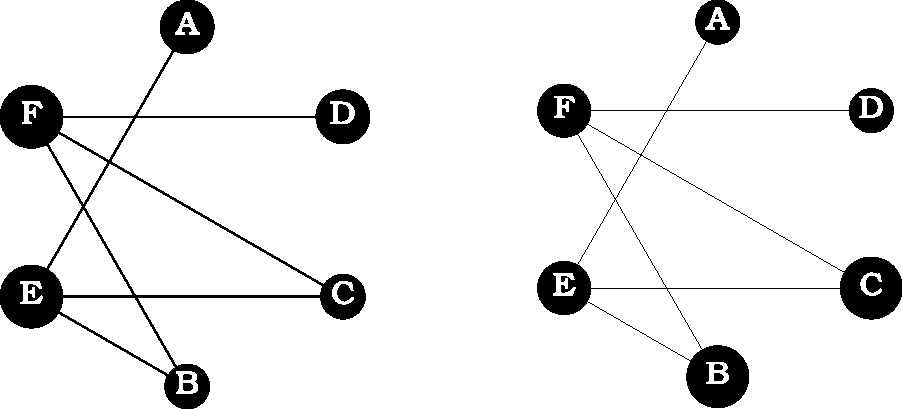
\includegraphics[scale=1]{img/graphs.pdf}
 		 \centering
 		 \caption{\textbf{$d$ \textit{(bal)} és TI\textsuperscript{2} \textit{(jobb)} szemléltetése ugyanazon a példagráfon} }
 		 A pontok átmérője arányos az adott nódusra kiszámolt $d$ (direkt vagy közvetlen topológiai kölcsönhatás) és TI$^2$ (topológiai fontosság két lépésre) értékekkel. \cite{ti} alapján módosítva.
 		 \label{fig:peldagraph}
 	 \end{figure}

 	 Az \ref{fig:peldagraph}. ábrán látható példagráfra rendre felírhatóak a közvetlen  kölcsönhatások ($d$) és a két lépésnyire közvetített indirekt kölcsönhatások ($d^2$) értékeit tartalmazó mátrixok:

	% Példamátrixok %
	\[
	\begin{blockarray}{ccccccc}
	&A & B & C & D & E & F \\
	\begin{block}{c [cccccc]}
	A &0 & 0 & 0 & 0 & \frac{1}{3} & 0 \\[6pt]
	B & 0 & 0 & 0 & 0 & \frac{1}{3} & \frac{1}{3}\\[6pt]
	C & 0 & 0 & 0 & 0 & \frac{1}{3} & \frac{1}{3}\\[6pt]
	D & 0 & 0 & 0 & 0 & 0 & \frac{1}{3}\\[6pt]
	E & 1 & \frac{1}{2} & \frac{1}{2} & 0 & 0 & 0\\ [6pt]
	F & 0 & \frac{1}{2} & \frac{1}{2} & 1 & 0 & 0\\ [6pt]
	\end{block}
	\multicolumn{7}{c}{\indent $d$ értékek} \\ [6pt]
	\end{blockarray},\quad
	\begin{blockarray}{ccccccc}
	&A & B & C & D & E & F \\
	\begin{block}{c [cccccc]}
	A & \frac{1}{3} & \frac{1}{6} & \frac{1}{6} & 0 & 0 & 0 \\[6pt]
	B & \frac{1}{3} & \frac{1}{3} & \frac{1}{3} & \frac{1}{3} & 0 & 0\\ [6pt]
	C & \frac{1}{3} & \frac{1}{3} & \frac{1}{3} & \frac{1}{3} & 0 & 0\\[6pt]
	D & 0 & \frac{1}{6} & \frac{1}{6} & \frac{1}{3} & 0 & 0\\[6pt]
	E & 0 & 0 & 0 & 0 & \frac{2}{3} & \frac{1}{3}\\ [6pt]
	F & 0 & 0 & 0 & 0 & \frac{1}{3} & \frac{2}{3}\\ [6pt]
	\end{block}
	\multicolumn{7}{c}{\indent $d^2$ értékek} \\[6pt]
	\end{blockarray}
	\]

	Az ábrázolt mátrixok elrendezése követi a populációdinamikai konvenciókat, tehát például $d_{BF}=\frac{1}{2}$ azt jelenti, hogy $F$ pont a $B$-re $\frac{1}{2}$ erővel hat. Mindkét mátrixra érvényes az, hogy az adott oszlop értékeinek összege egy. Ez a tulajdonság a $d$ érték definíciójából fakad. $d$ azt mutatja meg, hogy adott pont a cél pont kapcsolatainak hányad részét adja. Ezáltal minden pont egy egységnyi hatást kap ami eloszlik a vele kapcsolatban álló pontok között. \cite{ti} Ezt a hatást jól szemlélteti az \ref{fig:peldagraph}. ábra jobb oldali része amin látható, hogy $B$, $C$, $D$ és $A$ pontok kimenő hatása kisebb, mivel célpontjaik sok hatást fogadnak. \\
	\indent Ugyancsak mindkét mátrixra jellemző, hogy a sorok összege azt mutatja meg, hogy egy adott pont mennyire erős kölcsönható, tehát mekkora TI$^n$ értéke. Például $B$ pont két lépés távolságban összesen $\frac{4}{3}$ erővel hat, ez alapján erősebb kölcsönhatónak mondható mint az $A$ pont a maga $\frac{2}{3}$ értékű összesített kimenő két lépés hosszú hatásaival. \cite{ti} \\
	\indent Az \ref{fig:peldagraph}. ábrán az is jól megfigyelhető, hogy $C$ pont a gyengébb közvetlen kölcsönhatók közé tartozik. Ugyanakkor mivel a $C$-ből eredő két lépéses útvonalak erős elsődleges kölcsönhatókon keresztül érik el végpontjaikat, ezáltal két lépés távolság viszonylatában már $C$ is az erős kölcsönhatók közé tartozik. \\
	\indent Az $n > 1$ lépésszámú $d^n$ értékeket tartalmazó mátrixokban már egy adott pont indirekt hatása önmagára is kiterjedhet. Páros számú lépések esetén viszont mindenképpen felírhatók olyan útvonalak melyeken a pont eléri önmagát, \cite{ti} vagyis $d^n_{X,X} \neq 0$ ha n $\in$ \{ $2k :  k \in \mathbb{Z}$ \}. Az \ref{fig:peldagraph}. ábrán látszik, hogy például az $F$ pont két lépés távolságban a következű útvonalakon hat önmagára: $F \rightarrow B \rightarrow F$, $F \rightarrow C \rightarrow F$ és  $F \rightarrow D \rightarrow F$.

 	 \paragraph{Weighted Topological Importance - WI\textsuperscript{n}} \textcolor{red}{ !TODO}

\section{Célkitűzések}
	\paragraph{A diplomamunka célja} \mbox{}\\
	A diplomamunkám célja egy több adatbázisból integrált fehérje-fehérje kapcsolatokat tartalmazó humán-\textit{Salmonella} gazda-patogén hálózat létrehozása különböző adatbázisok alapján és az elkészült háló topológiai elemzése.


	Az elkészítendő hálózatnak a következőeket kell tartalmaznia:
	\begin{enumerate}
			\item Kurált \textit{H. sapiens} fehérje-fehérje kapcsolatok
			\item Kurált \textit{Salmonella} fehérje-fehérje kapcsolatok
			\item \textit{H. sapiens} és \textit{Salmonella} közti prediktált fehérje-fehérje kapcsolatok
	\end{enumerate}

	A topológiai elemzés során kapott adatok alapján véleményt szeretnék alkotni arról, hogy felhasználhatók-e az ökológiában fajok közti kapcsolatok vizsgálatára használt tisztán topológiai \DIFaddbegin \DIFadd{adatokon alapuló }\DIFaddend mérőszámok a molekuláris kapcsolati hálók elemzésére. Valamint, hogy az így előállított rangsorok mennyire korrelálnak a jelenleg használt \DIFdelbegin \DIFdel{\text{Salmonella} }\DIFdelend \DIFaddbegin \textit{\DIFadd{Salmonella}} \DIFaddend és humán bélsejteket vizsgáló módszerek eredményeivel.

	\paragraph{A célok eléréséhez tervezett feladatok}
	\begin{enumerate}
		\item Program írása mely képes az ARN (Autophagy Regulatory Network) adatbázis kurált humán autofágia specifikus fehérje-fehérje kapcsolati rétegének (``ARN core") MiTab SQL formátumra átalakítására.
		\item Program írása mely képes a Salmonet adatbázis kurált \textit{Salmonella} fehérje-fehérje kapcsolati hálózatának MiTab SQL formátumra átalakítására.
		\item Programok írása melyek képesek a Krishnadev és Skhirshagar féle humán-\textit{Salmonella} fehérje-fehéjre kapcsolati predikciók MiTab SQL formátumra alakítására.
		\item Program írása mely képes a létrehozott MiTab SQL fájlokban a fehérjék azonosítójának \textit{Uniprot} azonosítóra fordítására.
		\item Program írása mely képes a már csak \textit{Uniprot} azonosítókat tartalmazó adatbázisok összeejtésére.
		\item Program írása mely képes hálózatokban a megadott útvonalhosszra kiszámolni a topológiai fontosságot.
		\item A kapott adatsorok értékelése, hálózatok ábrázolása, biológiai relevancia keresése.
	\end{enumerate}

\section{Források és módszertan}

	\subsection{Informatikai módszerek}
			\paragraph{A problémák megoldására használt programnyelvek} \mbox{}\\
			A teljes adatbázisok feldolgozására valamint az adatbázisokból származó adatok rendszerezésére és megfelelő formátumúra alakítására \textit{Python} programnyelven írtam szkripteket. A diplomamunkám során a \textit{Python} 2.7-en és \DIFdelbegin \DIFdel{3-on }\DIFdelend \DIFaddbegin \DIFadd{3.4-on }\DIFaddend futtatható szkripteket \DIFdelbegin \DIFdel{is }\DIFdelend alkalmaztam. A fehérjék azonosítójának fordítását végző szkriptek egyike \DIFaddbegin \DIFadd{témavezetőm, }\DIFaddend Kadlecsik Tamás \textit{Javascript}ben írt fordítószkriptjének kismértékű módosítása.

			A diplomamunkám során alkalmazott szkriptek egy részét a \textit{Signalink} 3 szignalizációs adatbázis \DIFdelbegin \DIFdel{nulladik }\DIFdelend \DIFaddbegin \DIFadd{kézzel gyűlytött }\DIFaddend és \DIFdelbegin \DIFdel{harmadik rétegének }\DIFdelend \DIFaddbegin \DIFadd{külső adatokat tartalmazó rétegeinek (L0 és L3) }\DIFaddend létrehozásakor készítettem.  Mivel a \textit{Signalink} \DIFdelbegin \DIFdel{nulladik rétege }\DIFdelend \DIFaddbegin \DIFadd{rétegei }\DIFaddend is több adatbázisból integrál fehérje-fehérje interakciókat, így az ott alkalmazott munkafolyamat felhasználható volt a diplomamunkám gazda-patogén hálózatának létrehozásakor is. \textit{(\ref{fig:slk3uml}}. ábra) A humán-\textit{Salmonella} hálózat szerkezete azonban különbözik a \textit{Signalink} \DIFdelbegin \DIFdel{3 nullás rétegétől}\DIFdelend \DIFaddbegin \DIFadd{3-étól}\DIFaddend , mert például prediktált éleket is tartalmaz \DIFaddbegin \DIFadd{\textcolor{red}{Nem ez a legnagyobb különbség, inkább a fajok közti kapcsolatokat kellene említeni :D}}\DIFaddend . A két hálózat különbségei miatt, a diplomamunkámban az adatokat kezelő algoritmusok bár hasonlítanak a \textit{Signalink}et létrehozókra, de azokkal nem azonosak.

			 	 \begin{figure}[H]
			 		 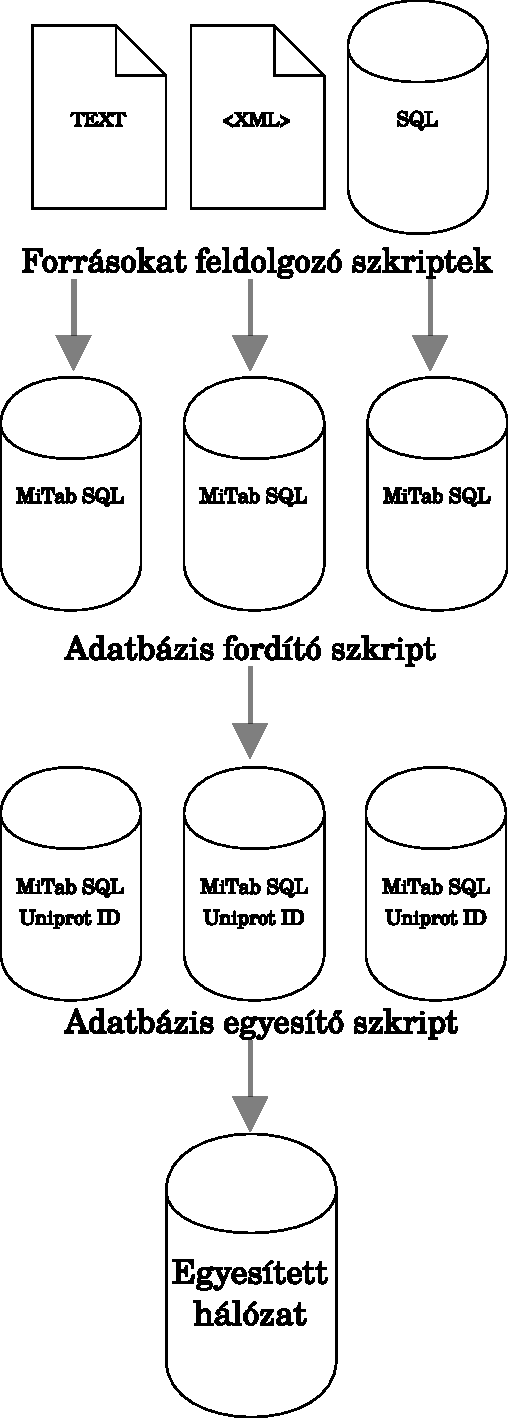
\includegraphics[scale=0.7]{img/Signalink_Layer0.pdf}
			 		 \centering
			 		 \caption{ \textbf{A hálózat létrehozásának folyamata} }
			 		 A különböző forrásokból származó adatok esetén először a forrás formátumokat feldolgozni képes szkriptek átalakítják azokat \DIFaddbeginFL \DIFaddFL{a belső szabványként használt }\DIFaddendFL MiTab SQL formátumra. Általában a különböző adatforrások különféle azonosítókkal illetik a komponenseiket. Ahhoz, hogy több hálózatot egyesíteni tudjunk, szükség van arra, hogy egy adott biológiai entitás csak egyfajta azonosítóval szerepeljen. A fordító szkript MiTab SQL fájlból olyan MiTab SQL fájlt \DIFdelbeginFL \DIFdelFL{gyárt}\DIFdelendFL \DIFaddbeginFL \DIFaddFL{készít}\DIFaddendFL , amiben az elsődleges azonosító már a kivánt, esetemben \textit{Uniprot} azonosító. Legvégül az adatbázis egyesítő szkript úgy ``összefűzi" a különböző hálózatok pontjait és éleit, hogy ne legyen benne redundáns információ.
			 		 \label{fig:slk3uml}
			 	 \end{figure}



			\paragraph{Az adatok tárolása} \mbox{}\\
			Az adatok ideiglenes tárolására, már a \textit{Signalink 3} készítése óta \DIFaddbegin \DIFadd{témavezetőm, }\DIFaddend Kadlecsik Tamás javaslatára \textit{SQLite 3} adatbázis fájlokat alkalmazunk.


			Az \textit{SQLite 3} egy nyílt forráskódú, \textit{C} nyelven írt API-val rendelkező, beágyazott relációs adatbázis motor. Az SQL sztenderd szintaxisának nagy részét tartalmazza. Sok népszerű programnyelv rendelkezik már beépített \textit{SQLite} támogatással, ilyen például a \textit{Python} is. \cite{sqlite3}


			Az adatok ilyen módú tárolása lehetővé teszi azok gyors szűrését, kategorizálását és átalakítását SQL parancsok segítségével. Ilyen módon még azelőtt gyorsan információkat nyerhetünk nagy méretű hálózatokról, mielőtt azokat olyan jóval lassabb működésű hálózatkezelő programokkal elemezni kezdenénk mint például a \textit{Cytoscape}. Az \textit{SQLite} adatbázisfájlok másik előnye, hogy rendelkezésünkre áll az SQL nyelv. Mivel SQL parancsok segítségével gyorsan kezelhetőek a feldolgozott adatok, így csak ritkán van szükség adatmanipulálási célból egy újabb szkript írására. Amennyiben mégis szükséges újabb szkript írása, a legtöbb szkriptnyelv rendelkezik valamilyen \textit{SQLite} adatbázis kezelési opcióval. Nagy méretű és mennyiségű biológiai adatot tároló \textit{SQLite} fájlban a keresés is igen gyorsan megoldható az adatbázis beindexelésével, sőt még gyorsabb keresés is megvalósítható az indexelt táblák memóriába csatolásával. Az \textit{SQLite} segítségével könnyen lehet importálni és exportálni a legtöbb népszerű adattárolási formátumba.

      \DIFaddbegin \DIFadd{Ezen indokok miatt használjuk a csoportomban az }\textit{\DIFadd{SQLite}} \DIFadd{adatbázisokat az adatok köztes tárolására, a szöveges fájlok helyett.
}

			\DIFaddend Hálózatok tárolására a csoport által létrehozott MiTab SQL formátumot használtam. A MiTab SQL egy \textit{SQLite 3}-ban tárolt a PSI-MI Tab formátummal közel megegyező adatstruktúra. A PSI-MI Tab egy \textit{HUPO Proteomics Standards Initiative} (PSI) szervezet által meghatározott proteomikai adatok tárolására használt formátum. A PSI-MI Tab formátum specifikációja a szervezet honlapján elérhető. \DIFaddbegin \DIFadd{\textcolor{red}{Hivatkozás! van hozzás cikk!}
}\DIFaddend 

			A pontok és az élek külön táblában vannak letárolva az adatbázisban, így a PSI-MI Tab specifikáció pontra és az élre vonatkozó tulajdonságai a megfelelő táblába kerülnek. A MiTab SQL táblák oszlopai azonban nem teljesen egyeznek a PSI-MI Tab kategóriákkal. Ilyen különbség például, hogy a MiTab SQL nem használ néhány opcionális PSI-MI kategóriát viszont tartalmaz a PSI-MI-re nem jellemző tulajdonságokat is mint a topológia. Az éleket tartalmazó táblában a forrás (\textit{interactor\_a\_node\_name}) és a cél pont név oszlopa a \textit{node} tábla azonosító oszlopának idegen kulcsai. (\ref{fig:mitab_scheme}. ábra)

				\begin{figure}[H]
					 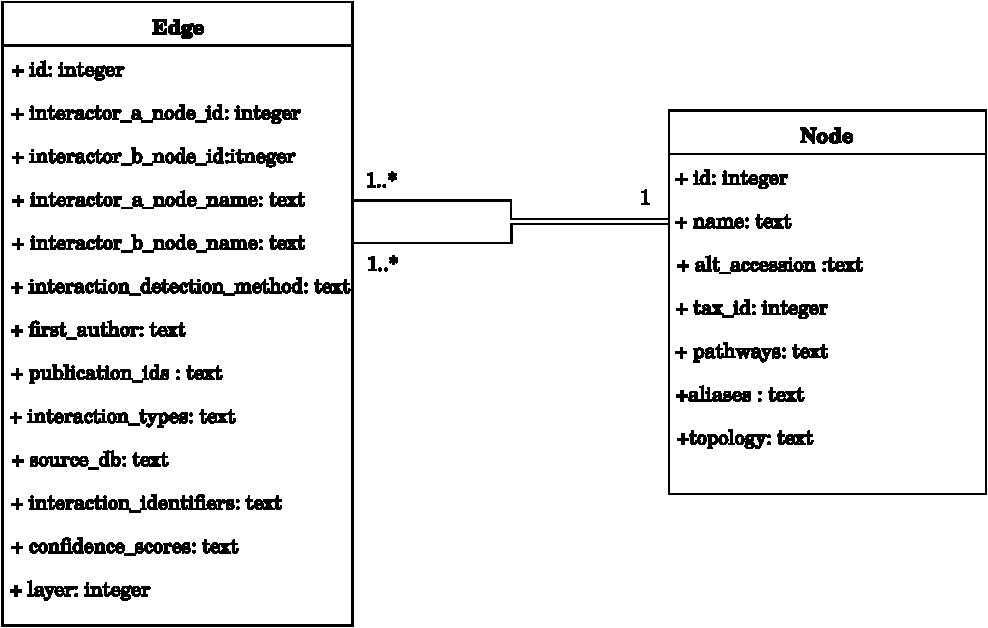
\includegraphics[scale=0.7]{img/Mitab-SQL.pdf}
			 		 \centering
			 		 \caption{ \textbf{A MiTab SQL sémája} }
			 		 \label{fig:mitab_scheme}
				\end{figure}

			\paragraph{Verziókövetés} \mbox{}\\
			Diplomamunkám készítése során a \textit{Git} verziókövető rendszert használtam, melynek tartalmát a web-alapú \textit{GitHub} tárhely szolgáltatásra töltöttem fel. A diplomamunkám GitHub tárhelyén (\ref{lst:github}. hivatkozás) a következő általam írt kódok érhetők el:
				\begin{itemize}
						\item A \ref{fig:slk3uml}. ábrán ábrázolt munkafolyamatot lebonyolító szkriptek
						\item A fordításhoz használt adatbázist megépítő szkript (Kadlecsik Tamás szkriptje alapján)
						\item A fordítást végző szkriptek
						\item Az adatbázisokat összeejtő szkriptek
						\item A MiTab SQL formátumot kezelő osztály
						\item A topológiai elemzést véző szkript
						\item Az adatszűrésre használt SQL szkriptek
				\end{itemize}

			\paragraph{Tesztelés}
			A bonyolultabb algoritmusok esetén \textit{egységteszteket (unit test)} alkalmaztam. A topológiai fontosságot kiszámító \textit{Python} osztály összes metódusának működését ilyen módon ellenőriztem. A teszteléshez a \textit{pyhthon} saját \textit{unittest} nevű csomagját használtam.



		\subsection{Az források feldolgozásának eszközei}

			\paragraph{MiTab SQLite adatbázis API} \mbox{}\\
			A \textit{PsimiSQL} egy \textit{Python} 2.7-es szintaxisban írt osztály, melyet még a \textit{Signalink 3} összeállításához \DIFdelbegin \DIFdel{kezdtem el készíteni}\DIFdelend \DIFaddbegin \DIFadd{készítettem}\DIFaddend , de azóta más projektekben is használtam és továbbfejlesztettem. A \textit{PsimiSQL} segítségével a molekuláris biológiai hálózatok könnyen átalakíthatók MiTab SQLite adatbázisokká. Az osztály számos függvényével megkönnyíti a MiTab SQLite adatbázisok kezelését \textit{Python} alól. Ilyen függvény például a redundáns adatok képzését gátló \textit{insert\_unique\_node()} mely ellenőrzi, hogy az adott hálózatban szerepel-e már az importálni kívánt pont. Az osztály példányosításakor a memóriában létrejön egy példányhoz kötött MiTab SQL sémával rendelkező SQLite 3 adatbázis. Az adatbázis benépesítése és az adatok keresése tehát nagy sebességgel történik. Az osztálynak vannak függvényei melyekkel könnyen importálni és exportálni lehet MiTab SQL adatbázis fájlokat.

			\paragraph{A szótárak építése és a fordítás} \mbox{}\\
			Ahhoz hogy a feldolgozott forrásokat össze lehessen fűzni egy nagy \DIFdelbegin \DIFdel{gráfba }\DIFdelend \DIFaddbegin \DIFadd{adat szettbe, }\DIFaddend szükség van arra, hogy a hálózatokban ne szerepeljen ugyanaz a biológiai entitás más azonosítóval. Ennek érdekében a mindegyik hálózat fehérjéit a legfrisebb \textit{Uniprot} adatbázis azonosítókra fordítottam. Ehhez két szkriptet kellett írnom.

			A Salmonet és az ARN már eleve \textit{Uniprot} azonosítókat használ. Azonban az \textit{Uniprot} adatbázis állandó frissítései miatt, fenn áll a lehetőség, hogy nem egy időben készült fájlok ugyanarra a fehérjére más \textit{Uniprot} azonosítót használnak. Egy másik hibaforrás az lehet, hogy a \textit{Uniprot} adatbázis egy fehérjét több azonosítóval is tárol. Előfordulhat, hogy egy fehérje többször is szerepel csak más \textit{Uniprot} azonosítókkal. Amikor egy fehérjét beletesznek a \textit{Uniprot} adatbázisba, akkor kap egy elsődleges azonosítót. Primer azonosítót kapnak még olyan fehérjék is, melyek már benne voltak az adatbázisban de később külön izoformákra lettek szétválasztva. Új elsődleges azonosítót kapnak olyan fehérjék is melyeket több vélt fehérjéből egyesítettek. Minden ilyen művelet után, a legfrissebb elsődleges azonosító marad az új elsődleges, az összes többi pedig másodlagos azonosítók lesznek. A \textit{Uniprot} azonosítókat még csoportosítani lehet az alapján is, hogy a fehérje manuálisan vagy automatikusan lett annotálva. Az első típusba az úgynevezett \textit{Swissprot} az utóbbiba pedig a \textit{trEMBL} azonosítók tartoznak. Minden swissprot azonosító egyben elsődleges azonosító is \DIFaddbegin \DIFadd{\textcolor{red}{ez tuti? van rá forrás?}}\DIFaddend . A szkriptem az összes pont azonosítójára, ha az nem \textit{Swissprot}, kikeresi a swissprot azonosítót ha létezik, vagy az elsődleges trembl azonosítót. Az ARN és a Salmonet fordításához szükség volt egy \textit{Salmonella}-\textit{Salmonella} és egy humán-humán szótárra, amiket a Kadlecsik Tamás féle szótárépítő scripttel állítottam elő. Az azonosítókat a szótárak alapján saját készítésű szkripttel fordítottam.

			A predikciókhoz egy olyan szótárat kellet létrehozni, mely \textit{Salmonella} génazonosítókhoz rendel \textit{Salmonella} \textit{Uniprot} azonosítókat \DIFaddbegin \DIFadd{\textcolor{red}{na itt ki kellene fejteni hogy ez miért kell}}\DIFaddend . Ezt szintén Kadlecsik Tamás szkriptjével állítottam elő. Egy általam írt másik fordítószkript segítségével pedig az előzőhöz hasonló módon fordítottam a predikciókat.


		\subsection{A források}
			\subsubsection{Autophagy Regulatory Network (ARN)}
			Az ARN egy széles terjedelmű autofágia adatbázis. Az adatbázis az irodalomból kézi gyűjtéssel kapott élek mellett tartalmaz még 19 más adatbázisból importált valamint 4 féle predikcióval készült feltételezett kapcsolatokat is. Az ARN-ben található 1485 darab fehérje között 4013 kapcsolat van. Az adatbázis komponensei között vannak az autofágia mechanizmusában szerepet játszó fehérjék és ezek regulátorai valamint transzkripciós faktorai. Az adatbázisban 413 transzkripciós faktor valamint 386 olyan miRNS melyek képesek lehetnek autofágia komponensek szabályzására.\cite{ARN} \\
			Az ARN hat rétegből épül fel:
			\begin{enumerate}
				\item Autofágia fehérjék.
				\item Az első réteg fehérjéinek autofágia specifikus forrásokból származó regulátorai.
				\item Olyan poszt-transzlációs regulátorok melyek közvetlenül hatnak az első két réteg fehérjéire.
				\item Az első három réteg transzkripciós szabályzói.
				\item Az első négy réteg poszt-transzlációs regulátorai.
				\item Olyan jelátviteli útvonalak és fehérje-fehérje interakciók melyek különböző útvonalakat az autofágia szabályzókhoz kötnek.
			\end{enumerate} \cite{ARN}

			\paragraph{Az ARN feldolgozása} \mbox{}\\
			A gazda patogén hálózat összeállításához az ARN adatbázisnak csak az első, autofágia fehérjéket tartalmazó rétegét használtam fel. A hálózat letöltését követően azt egy általam írt \textit{Python} scripttel MiTab SQL formátumba alakítottam. A fordító szkripttel az akkor legfrissebb \textit{Uniprot} adatbázis azonosítókra fordítottam. \DIFaddbegin \DIFadd{\textcolor{red}{ide kellene egy minimális megjegyzés hog yakkor amikor az arn készült még nem használtuk ezt a belső szabványt}
}\DIFaddend 

			\subsubsection{Salmonet}
			A \textit{Salmonet} a csoportunk által készített de még nem publikált molekuláris hálózat. A háló kézi gyűjtésű \textit{Salmonella-Salmonella} fehérje-fehérje kapcsolatokat tartalmaz.

			\paragraph{A Salmonet feldolgozása} \mbox{}\\ \DIFaddbegin \DIFadd{\textcolor{red}{ezek szándékosan számozatlan alfejezetek?}
			}\DIFaddend Az \textit{Salmonet} átalakítása az ARN-hez hasonló módon történt, azzal a különbséggel, hogy fordításkor \textit{Salmonella}-\textit{Salmonella} szótárat használtam. \DIFaddbegin \DIFadd{\textcolor{red}{ide majd kellene egy in prep. hivatkozás}
}\DIFaddend 

			\subsubsection{A predikciók}
			Az eddig ismertetett források csak fajon belüli kapcsolatokból felépülő hálózatokat tartalmaztak. Ahhoz, hogy szakdolgozatomban tudjam tanulmányozni a humán-\textit{Salmonella\DIFdelbegin \DIFdel{kapcsolatot}\DIFdelend } \DIFaddbegin \DIFadd{kapcsolatot }\DIFaddend szükségem van még interspecifikus élekre is. A predikciós forrásokból származó interspecifikus kapcsolatok fogják összekapcsolni a gazda hálózatát a patogénével. Szakdolgozatomban \cite{Krishnadev} és \cite{Kshirsagar} humán-\textit{Salmonella} predikcióit használtam.

			\paragraph{A predikciók feldolgozása} \mbox{}\\
			A két predikció feldolgozására külön \textit{Python} szkripteket írtam. Csakúgy mint az előző forrásokat, az így elkészült adatbázisokat a legújabb \textit{Uniprot} azonosítóra fordítottam.




	\subsubsection{Az adatbázisok egyesítése}
		Az adatbázisok egyesítésekor a fő szempont az, hogy az végleges hálózatban ne legyenek redundáns pontok vagy élek. Az adatbázis egyesítő szkript beolvassa az összes adatbázisfájlt és eg \textit{has-map}ben eltárolja a pontokat és éleket és ezek tulajdonságait. A \textit{hasm-map}-ből gyorsan ki kereshető, hogy egy adott él vagy pont benne van-e már \DIFaddbegin \DIFadd{\textcolor{red}{ide jó lenne egy megjegyzés hogy sokkal gyorsabb mint az sqlite}}\DIFaddend . Ami a szkript végigmegy az összes adatbázisfájlon a \textit{has-map}-ek tartalmából létrehoz egy MiTab SQL fájlt mely nem redundánsan tartalmazza az összes forrás adatbázis tartalmát.

	\subsection{A hálózatok topológiai elemzése}

		\subsubsection{A TopologyAnalyser osztály}
		A \textit{TopologyAnalyser} osztály \textit{Python 3} szintaxist használ. Az osztály segítségével kiszámítható a Jordán Ferenc féle topológiai fontosság (TI$^n$). Az TopologyAnalyser egyetlen külső függősége a NetworkX csomag. A NetworkX egy \textit{Python}ban írt, komplex hálózatok létrehozására, manipulálására és elemzésére használható ingyenes csomag. \DIFaddbegin \DIFadd{\textcolor{red}{ide gyorsan leírhatnád hogy a másik két graph csomag helyet miért ezt használtad}
}\DIFaddend 

		Az osztály konstruktorának egyetlen paramétere egy éllista. Példányosítás után a \textit{TopologyAnalyser} típusú objektum, egy éllistát, egy \textit{Graph} típusú objektumot és egy egység-élerősségi mátrixot tartalmaz.

		A \textit{Graph} osztály a NetworkX csomag része és irányítatlan gráfok tárolására alkalmas. A hálózat példányhoz kötött \textit{Graph} típusú objektum (\textit{self.graph}) tárolása előnyös, mert így elérhetők a NetworkX csomag különböző gráf elemzésre használható metódusai. Ilyen függvény például a \textit{Graph.neighbors\_iter(node)} mely egy adott pont szomszédjainak iterálható listáját adja vissza.

		Az élerősség mátrix (\textit{self.edgeStrength}) egy példányhoz kötött \textit{Python Dictionary}. A \textit{Dictionary} osztály   \textit{Pythonban} \textit{hashmap} adatstruktúrával van implementálva, ezáltal a benne tárolt adatok gyorsan elérhetők. A szótár kulcsai a mátrix indexei, az értékei pedig az élerősségek \textit{Fraction} típusú objektumokként letárolva. Az egységerő mátrix celláinak indexei maguk az élt alkotó pontok \textit{Uniprot} azonosítói. Az élerősség mátrix 0 értékkel rendelkező cellái nincsenek letárolva a \textit{hasmap}-ben.

		\paragraph{Az osztály fontosabb metódusai és működésük}

		\begin{itemize}
			\item \textit{getNthNeighbors()}

			A függvény rekurzívan kikeresi az adott pont $n$. szomszédját.

			\item \textit{pathFinder()}

			Ez a függvény megkeresi az összes $n$ hosszúságú útvonalat egy forrás és egy cél nódus között.

			  		\begin{algorithm}[H]
						\footnotesize

						\SetAlgoVlined
						\SetKwProg{Def}{def}{:}{}
						\Def{pathfinder(mélység, forrás nódus, cél nódus, útvonal, összegyűjtött útonalak)}{
							\uIf{útvonalhossz == 0}{
														forrás nódus hozzáadása az útvonalhoz \;
														mélység =- 1
													}
													\uElseIf{mélység == 0 és forrás nódus == cél nódus}{
														\Return útvonal
													}
													\ElseIf{mélység == 0 és forrás nódus $\neq$ cél nódus}{
														\Return
													}

													\For{forrás nódus első szomszédai}{
														szomszéd nódus hozzáadása az útvonalhoz\;
														pathfinder( mélység - 1, szomszéd nódus, cél nódus, útvonal, összegyűjtött útvonalak) \;
														az utolsó pont eltávolítása az útvonalból\;
													}
						}



			  		\end{algorithm}

			\item \textit{buildEdgeUnitStrengthDict()}

			Ez a függvény egyszer hívódik meg a konstruktor lefutása során. A metódus imperatív módon egy \textbf{for} ciklussal \DIFdelbegin \DIFdel{végigmegy }\DIFdelend \DIFaddbegin \DIFadd{végig iterálja }\DIFaddend a kapott éllistán. A függvény visszatérési értéke egy egységerő mátrix.

			\item \textit{getNthPathwaysForNodes()}

			A függvény először minden pontnak megkeresi az $n$. szomszédját.  Mint az irodalmi bevezetőben ismertettem, a topológiai fontosság számolásánál páros lépésszámnál hurkon keresztül egy adott pont mindig önmagának a szomszédja is. A metódus két egymásba ágyazott \textbf{for} ciklust használ. A külső ciklus minden ponra előállítja a pont $n$. szomszédjainak halmazát. A belső ciklus pedig minden cél és forrás pont párra meghívja a \textit{pathFinder()} függvényt, majd a kapott útvonalakat imperatívan hozzáadja egy listához, amit még a ciklusokon kívül definiáltam. A metódus visszatérési értéke egy lista amelyben minden lehetséges forrás és célpont közötti $n$ hosszúságú útvonal benne van.

			\item \textit{getEdgesFromPathway()}

			A metódus egy útvonalat fogad és az azt alkotó élek listájával tér vissza.

			\item \textit{countPathwayStrength()}

			A metódus egy útvonalat kap, amire meghívja a \textit{getEdgesFromPathway} függvényt. A kapott éllistán végigmegy és minden élre kikeresi az egységerő mátrixból a megfelelő értéket. Az összes él erejének összeszorzása után az út erősségével tér vissza.

			\item \textit{getPathWaysToNthNeighbours()}

			Ez a függvény kikeresi egy adott pont összes $n$. szomszédját és egy listában letárolja. Amikor elkészült a szomszédok listájával, akkor ezen egy \textbf{for} ciklus segítségével végigmegy. Ekkor minden periódusban meghívja a forrás és az aktuális cél nódusra a \textit{pathfinder} függvényt, majd a kapott útvonalakat imperatíven hozzáfűzi egy a cikluson kívül definiált listához. A ciklus után a függvény visszatér az elkészül listával.

			\item \textit{countTI()}

			A függvény egy adott pontra meghatározza annak topológiai fontosságát. Első lépésként létrehoz egy útvonal listát a \textit{getPathWaysToNthNeighbours} metódus segítségével, majd végigmegy az útvonalak listáján egy \textbf{for} ciklusban. Minden periódusban meghívja a \textit{countPathwayStrength(pathway)} függvényt az aktuális útvonalra, és annak eredményét egy a cikluson kívül definiált változóba akkumulálja.

		\end{itemize}

\section{Eredmények (A hálózat elemzése)}
	\subsection{Főbb statisztikák}
	\subsection{Kapott topológiai adatok és jelentésük}

\section{Diszkusszió}
\section{Összefoglalás}
\section{Summary}
\section{Hivatkozások jegyzéke}
	1. link \textcolor{red}{TODO github link} \label{lst:github}
\section{Köszönetnyilvánítás}
\section{Nyilatkozat}

\pagebreak


\bibliography{msc_szakdolgozat}{}
\bibliographystyle{apalike}

\end{document}
